\chapter{Electrones identificados como fotones}\label{ch:e_fake}
\chaptermark{Electrones identificados como fotones}


Como ya se mencionó anteriormente, existe un fondo que contribuye a procesos asociados a fotones y jets como estado final, donde un electrón del estado final es identificado como un fotón. Este puede provenir de procesos del SM, como los que producen bosones W y Z + jets, y $t \overline{t}$. El mismo es difícil de estimar a partir de simulaciones, ya que dependen en gran medida de la estructura y material del detector que es muy compleja de modelar en todos sus detalles. El objetivo es entonces estimar este fondo calculando un factor de identificación errónea (\textit{Fake Factors}) en función de las variables $\eta$ y $p_{T}$ de los objetos a partir de los datos adquiridos.

\section{Medición del factor de identificación errónea}

El metodo para la estimación del factor de identificación errónea, hace uso de la muestra de eventos $Z\rightarrow ee$. En base a esta muestra, se determinan la relación de eventos de pares electrón-positrón y los paras electrón(positrón)-fotón cuya masa invariante es compatible con la del bosón $Z$. Estos últimos pares así selecionados provienen de eventos en los cuales un electrón (positrón) del decaimiento del $Z$ es reconstruído como un fotón. El factor de identificación espuria se puede calcular entonces como: 

\begin{equation}
F_{e\rightarrow\gamma}[\eta , p_{T}]=\frac{N^{eg}[\eta , p_{T}]}{N^{ee}[\eta , p_{T}]} \label{eq:ff_ratio}
\end{equation}

Como la muestra de pares de objetos seleccionada no es una muestra pura de $Z\rightarrow ee$, se realiza un ajuste a la distribución de su masa invariante para determinar por separado la contribución de señal y de fondo en cada muestra, como se explicará más adelante.

Los criterios para selecionar los objets de los pares de partículas mencionados se explican a continuación y se basan en criterios de selección que mantengan una alta pureza de la muestra, manteniendo un bajo rechazo de señal.
Los electrones  son seleccionados con $p_{T} > 25 \egev$, con un criterio de calidad \textit{tight} y punto de trabajo de aislamiento denominado \textit{gradient loose} \cite{ATLAS-CONF-2016-024}. Para los fotones los requisitos son $p_{T} > 25 \egev$, \textit{tight} y aislados \cite{STDM-2010-08}. A ambos se les solicita que tengan un $\eta_{BE}<2.37$, que estén fuera de la region del \textit{crack} entre $1.37$ y $1.52$, que provengan del vértice primario en base a un parámetro de impacto $d_{0}$ con una significancia menor a 5, y que cumplan con la relación $|\Delta z_{0}sin\theta|<5$.

Además, si un electrón y un fotón son reconstruidos con $\sqrt{\Delta\phi^{2}+\Delta\eta^{2}}<0.4$, el fotón es descartado del evento. Esto reduce precisamente la probabilidad de utilizar candidatos donde un electrón es reconstruido como fotón. 

A todos los pares se les solicita que una masa invariante entre $75$ y $105 \egev$  estando así en la region de cercanía a la masa del $Z$. Finalmente, en el caso de que existiese más de un par en el evento, se utiliza el que tiene la masa invariante más cercana a la del bosón $Z$ ($91.1876 \pm 0.0021 \egev$\cite{Olive:2016xmw}). Ya que esto minimiza la contaminación de pares aleatorios, descartando solo unos pocos eventos donde pueda haber más de un $Z$ en estado final.


En base a los objetos selecionados se crea un arreglo bidimensional en  $\eta$ y $p_{T}$. Para eventos positrón-electrón una entrada se realiza para cada partícula. En los casos de pares electrón-fotón un arreglo es creado por separado y los solo los valores de los fotones son utilizados.

La concepción del método proviene de la siguiente consideración. Sea $\epsilon_{i}$ la eficiencia de reconstruir un electrón, con un valor de $\eta$ y $p_{T}$ correspondientes al bin \textit{i} del histograma. Para una muestra de \textit{N} pares de electrones y positrones reales (dentro del rango de masa), decimos que $f_{ij}$ es la fracción de pares para los cuales el electrón \textit{leading} (\textit{sub-leading}) está dentro del bin \textit{i} (\textit{j}). Considerando solamente electrones-positrones provenientes del decaimiento de un bosón Z, el número de eventos en el bin \textit{i} del histograma $N^{ee}[\eta , p_{T}]$ es entonces:

\begin{equation}
N_{i}^{ee} = \sum_{i}\epsilon_{i}\epsilon_{j}f_{ij}N + \sum_{j}\epsilon_{j}\epsilon_{i}f_{ji}N = \epsilon_{i}N\sum_{j}\epsilon_{j}(f_{ij}+f_{ji})
\end{equation}

De forma análoga, ahora considerando que $p_{i}$ es la proporción de fotones reconstruídos como electrones en el bin \textit{i}, la cantidad de eventos en el bin \textit{i} del histograma $N^{eg}[\eta , p_{T}]$ es:

\begin{equation}
N_{i}^{eg} = \sum_{i}p_{i}\epsilon_{j}f_{ij}N + \sum_{j}p_{j}\epsilon_{i}f_{ji}N = p_{i}N\sum_{j}\epsilon_{j}(f_{ij}+f_{ji})
\end{equation}

El factor que determina la proporción de electrones reconstruidos como fotones se define finalmente como:

\begin{equation}
F_{e\rightarrow\gamma}[\eta , p_{T}]\equiv\frac{N^{eg}}{N^{ee}}=\frac{p_{i}}{\epsilon_{i}}
\end{equation}

Por ende, el factor, no es la proporción de fotones mal reconstruidos, sino que es el cociente entre esa proporción y la eficiencia de reconstruir un electrón. De esta forma el fondo correspondiente a electrones identificados como fotones resulta:

\begin{equation}
N_{e\rightarrow\gamma}(\eta , p_{T} , ... )=F_{e\rightarrow\gamma}(\eta , p_{T})\cdot N_{e}(\eta , p_{T} , ...)
\end{equation}
	
Donde $N_{e}(\eta , p_{T} , ...)$ es el número de electrones en un determinado estado final.

La implementación del cálculo en ROOT y C++ se  base en histogramas bidimensionales. Para cada evento que contiene un par electrón-positrón, en un histograma con bines de $\eta$ y $p_{T}$ ($N^{ee}[\eta , p_{T}]$), se suma una entrada en el bin correspondiente al $\eta$ y $p_{T}$ de cada uno de los electrones. En el caso de que el evento tenga un par electrón-fotón, en otro histograma ($N^{eg}[\eta , p_{T}]$), se suma una entrada en el bin correspondiente al $\eta$ y $p_{T}$, solamente del fotón. El correspondiente factor se obtiene entonces como en la ecuación \ref{eq:ff_ratio}.

Para tener en cuenta la relación entre entradas correspondientes a la señal y las correspondientes al fondo, cada entrada en los histrogramas es pesada con un peso que tiene en cuenta esta relación. Este peso se obtiene clasificando a los pares según el tipo ($ee-e\gamma$) y según la región donde se reconstruían los objetos ($EE-BE-BB$). Para cada uno se calcula su masa invariante, y finalmente el peso resulta de la relación entre señal (S) y fondo (B): $w=\frac{S}{S+B}$. Esto se debe a que los pares tienen un probabilidad de no provenir del decaimiento del bosón $Z$, sino de otros procesos no resonantes de fondo. La relación entre señal y fondo tiene en cuenta esta probabilidad.

Los datos utilizados para el análisis corresponden al Run 1 y al Run 2 del LHC, con una derivación EGAM1 y con ningún requisito de \textit{triggers}. Para los ajustes de la masas invariantes se utiliza como modelo de señal una \textit{double-sided Crystall-ball} (DSCB). Para el fondo se utiliza un polinomio de grado 2. Los resultados de los ajustes obtenidos para cada clasificación de los pares se pueden observar en las Figuras \ref{fits_BB}, \ref{fits_BE} y \ref{fits_EE}.

Se consideran distintas fuentes de incertezas sistemáticas. Una de ellas proveniente de la variación tanto del rango del fit, como del rango de masa de aceptación de los pares. El rango nominal del fit es $[70-110]\egev$ y se varía a $[65-115]\egev$ y a $[75-105]\egev$. El rango nominal de la masa es $[75-105]\egev$ y se varía a $[70-110]\egev$ y a $[80-100]\egev$. Se tuvo en cuenta también como fuente de sistemático, la variación en los valores de los factores al utilizar otra función para el ajuste del fondo, utilizándose un polinomio de grado 3 y un polinomio de Bernstein de grado 4.

Los resultados obtenidos para el factor en bines de $\eta , p_{T}$ se muestran en la tabla \ref{fftable}.

\begin{table}	
\centering
\begin{threeparttable}
\caption{Tabla con los factores de identificación errónea en bines de $\eta$ y $p_{T}$, con sus valores de incerteza estadística y sistemática.}
\begin{tabular}{ l l c c c c c c }

	\hline
	\hline

	\multirow{2}{*}{$|\eta|$} & \multirow{2}{*}{$p_{T}$[GeV]} & \multirow{2}{*}{Fake factor} & \multirow{2}{*}{Estad.} & \multicolumn{4}{c}{Sistemáticos} \\

	\cline{5-8}

	 & & & & Bern 4$\degree$ & Poli 3$\degree$ & Rango & Total \\


	\hline

	0 - 0.6 & 75 - 90 & 0.0168 & 0.0003 & -			& 0.0003  &  0.0004 &  0.0006  \\

	0 - 0.6 & 90 - 145 & 0.0158 & 0.0004 & - 		& 0.0002  &  0.0003 &  0.0005  \\

	0 - 0.6 & 145 - 300 & 0.0142 & 0.0007 & -  		& 0.0002  &  0.0003 &  0.0008  \\

	\hline

	0.6 - 1.37 & 75 - 90 & 0.0186 & 0.0003 & -		& 0.0002  &  0.0004 &  0.0005  \\

	0.6 - 1.37 & 90 - 145 & 0.0183 & 0.0004 & -		& 0.0002  &  0.0004 &  0.0006  \\

	0.6 - 1.37 & 145 - 300 & 0.0141 & 0.0007 & -  	& 0.0002  &  0.0003 &  0.0008  \\

	\hline

	1.52 - 1.82 & 75 - 90 & 0.0354  & 0.0009 & -		& 0.0003  &  0.001 &  0.001  \\

	1.52 - 1.82 & 90 - 145 & 0.033  & 0.001 & -		& 0.001  &  0.001  &  0.002 \\

	1.52 - 1.82 & 145 - 300 & 0.026  & 0.002 & -  	& 0  &  0.0005  &  0.002  \\

	\hline

	1.82 - 2.37 & 75 - 90 & 0.045  & 0.001 & -		& 0.0001  &  0.001 &  0.001  \\

	1.82 - 2.37 & 90 - 145 & 0.040  & 0.001 & -		& 0.001  &  0.002  &  0.002  \\

	1.82 - 2.37 & 145 - 300 & 0.038  & 0.002 & -  	& 0  &  0.002  &  0.003  \\

	\hline
	\hline

\end{tabular}
\label{fftable}
\end{threeparttable}
\end{table}


\begin{figure}

	\begin{subfigure}{0.5\textwidth}
		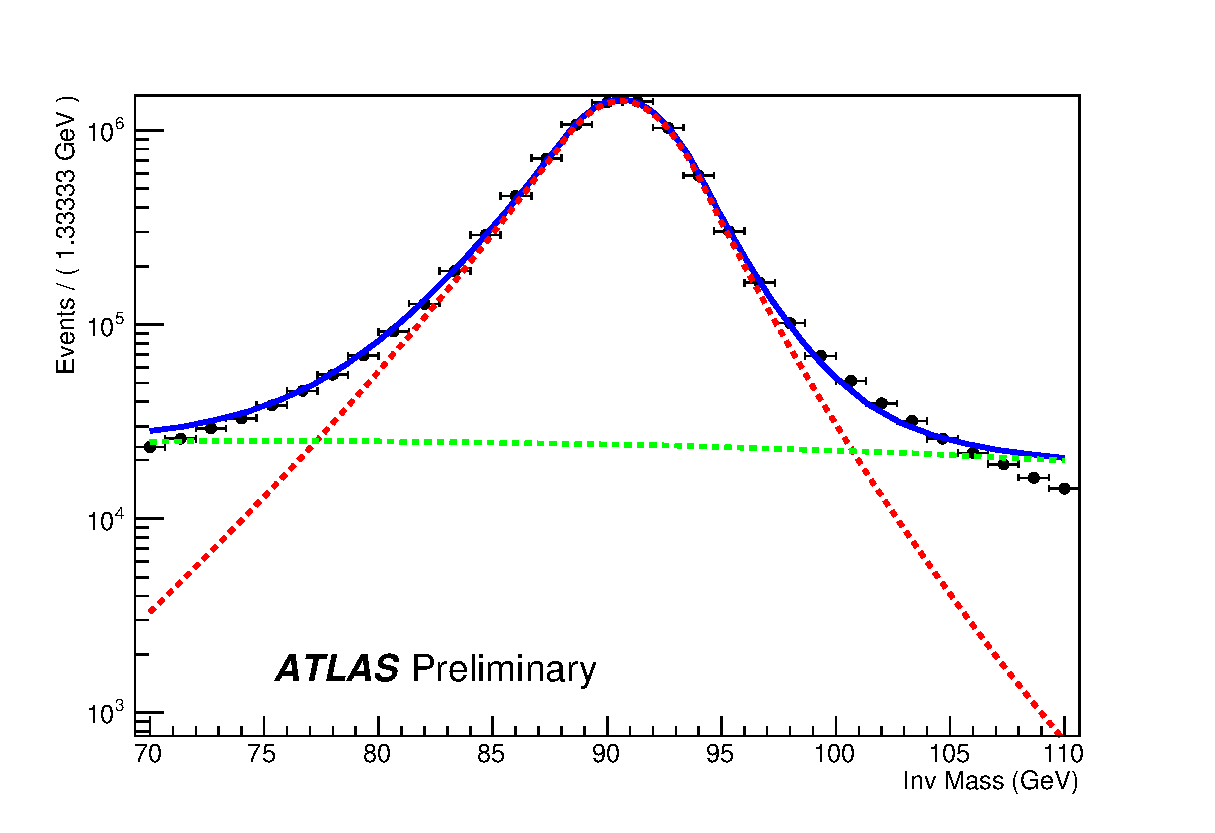
\includegraphics[scale=0.40]{d15_16_egam1_m_fit_h_m_ee_BB.eps} 
	\end{subfigure}
	~
	\begin{subfigure}{0.5\textwidth}
		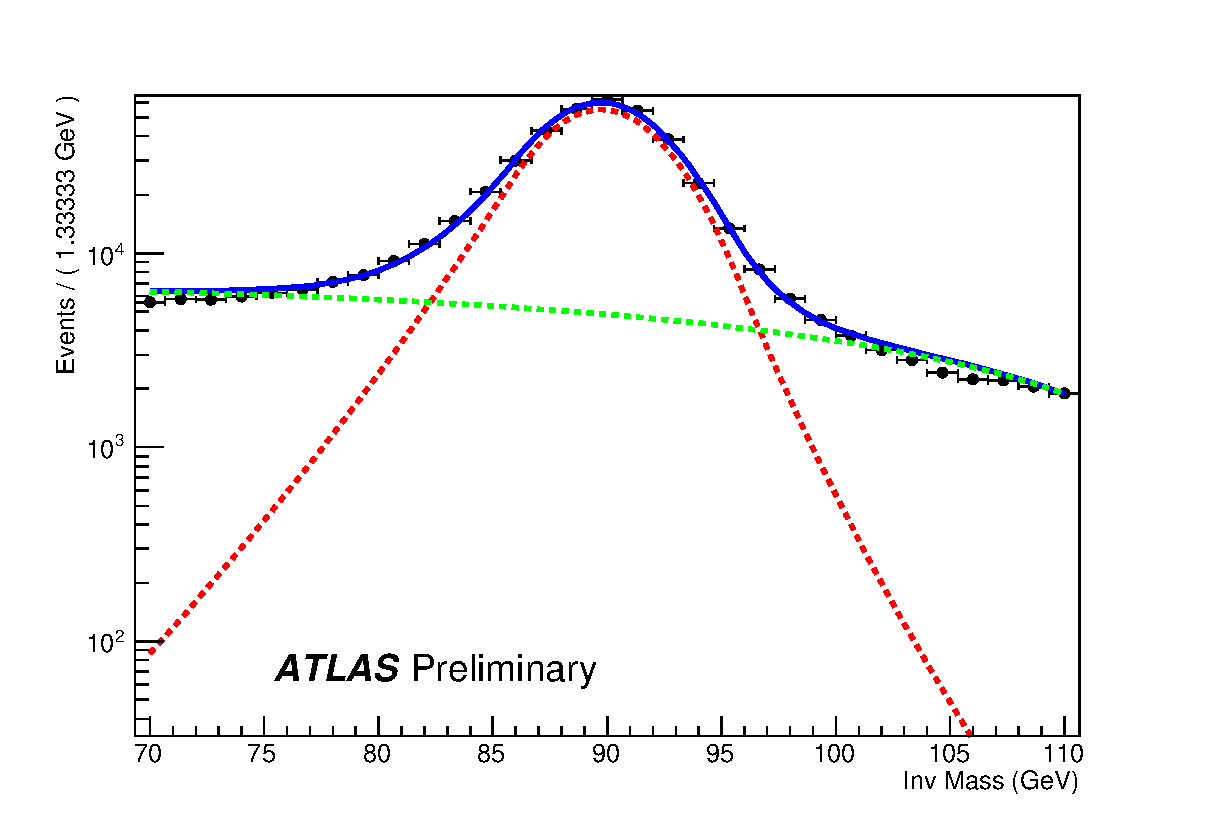
\includegraphics[scale=0.40]{d15_16_egam1_m_fit_h_m_eg_BB.eps}
	\end{subfigure}

	
	\caption{Fits de la masa invariante de los pares $ee$ (izquierda) y $e\gamma$ (derecha), reconstruídos en al región $BB$. La curva roja corresponde a la DSCB, la verde al polinomio de grado 2 y la azul a la combinación resultante de ambas.}
\label{fits_BB}
\end{figure}

\begin{figure}

	\begin{subfigure}{0.5\textwidth}
		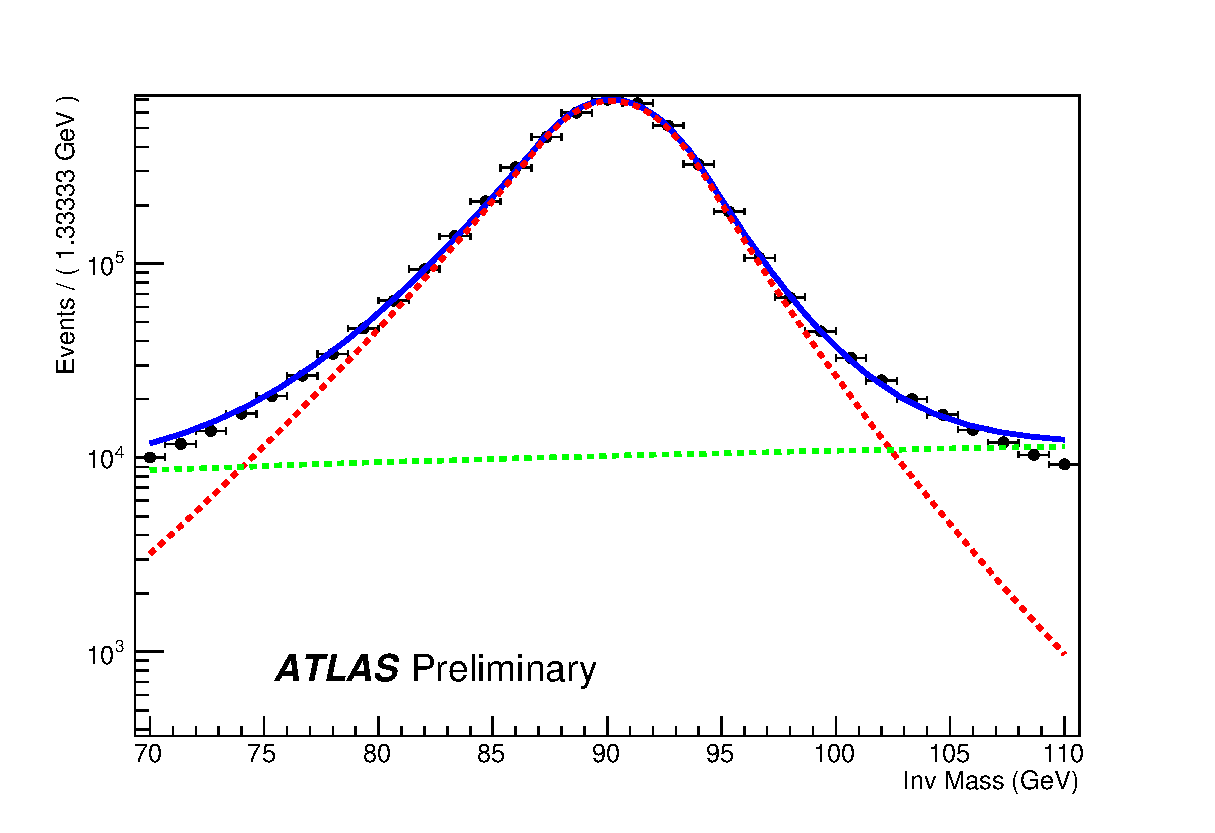
\includegraphics[scale=0.40]{d15_16_egam1_m_fit_h_m_ee_BE.eps} 
	\end{subfigure}
	~
	\begin{subfigure}{0.5\textwidth}
		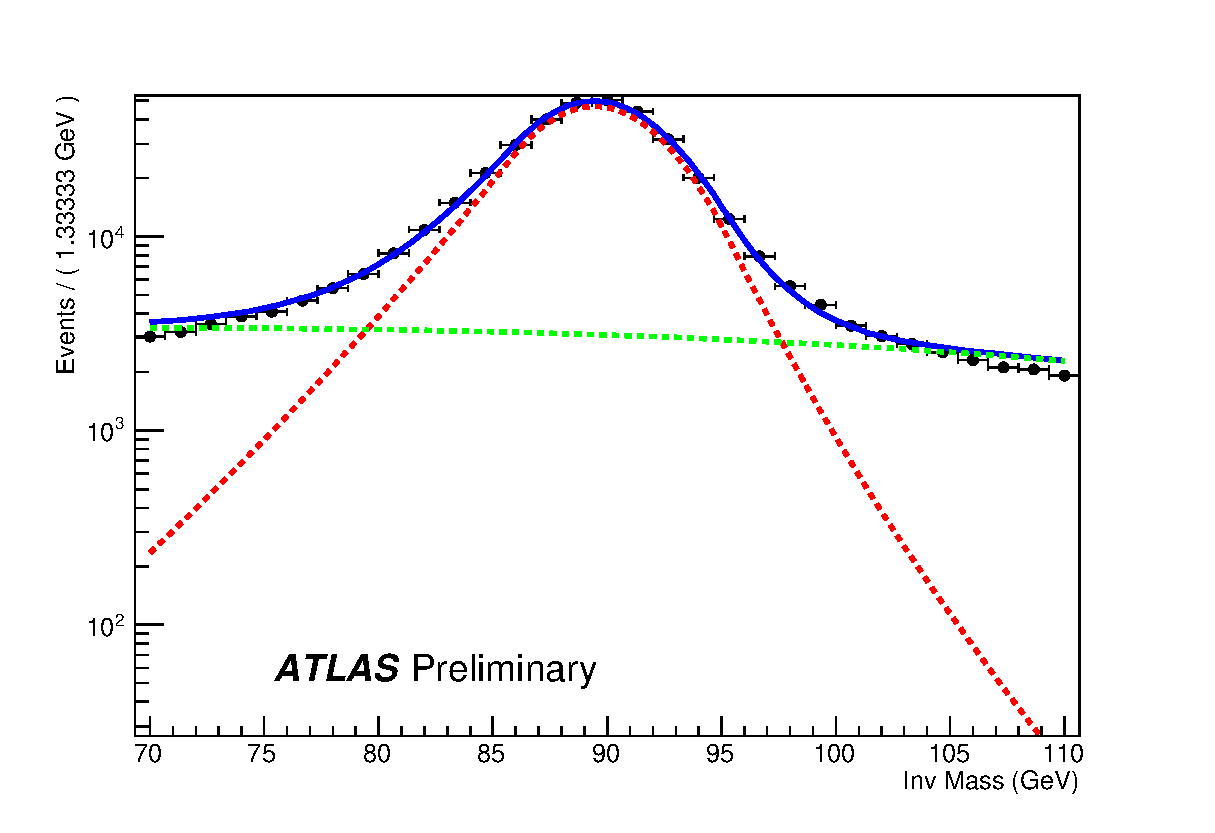
\includegraphics[scale=0.40]{d15_16_egam1_m_fit_h_m_eg_BE.eps}
	\end{subfigure}

	
	\caption{Fits de la masa invariante de los pares $ee$ (izquierda) y $e\gamma$ (derecha), reconstruídos en al región $BE$. La curva roja corresponde a la DSCB, la verde al polinomio de grado 2 y la azul a la combinación resultante de ambas.}
\label{fits_BE}
\end{figure}


\begin{figure}

	\begin{subfigure}{0.5\textwidth}
		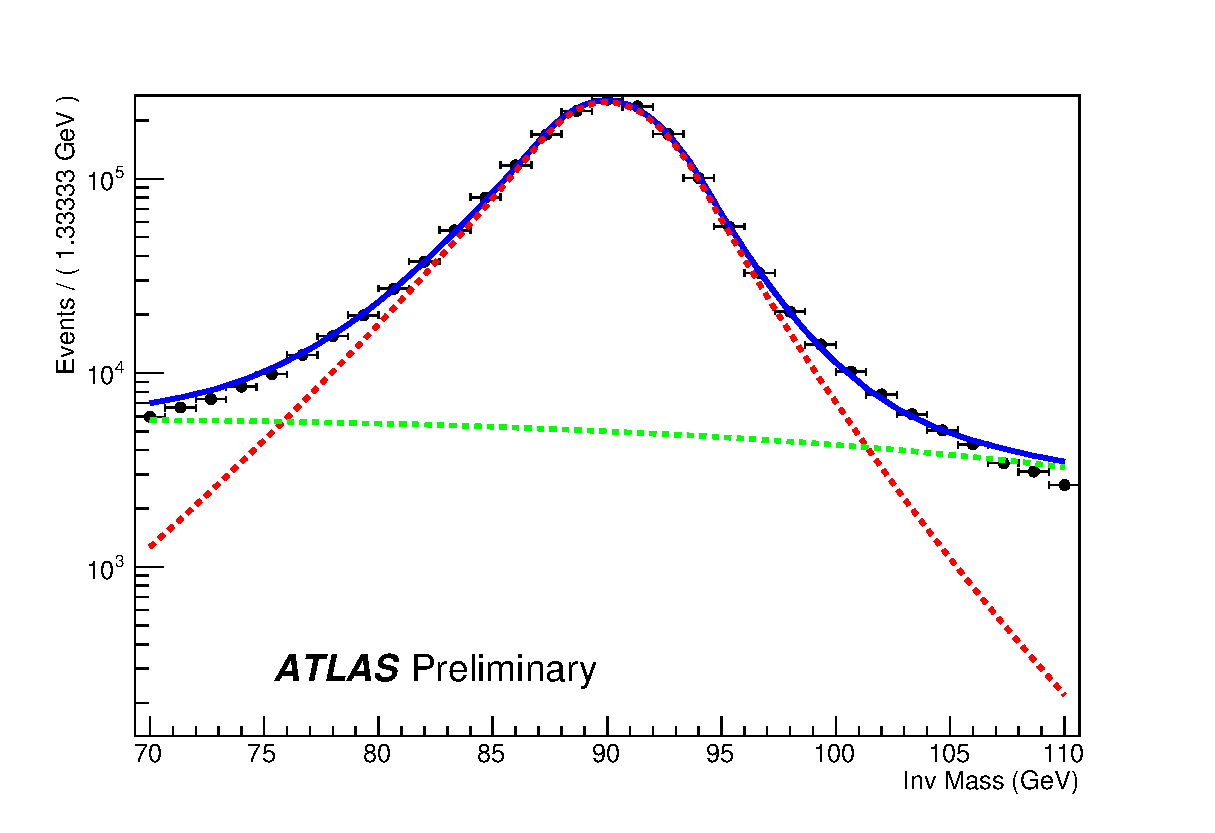
\includegraphics[scale=0.40]{d15_16_egam1_m_fit_h_m_ee_EE.eps} 
	\end{subfigure}
	~
	\begin{subfigure}{0.5\textwidth}
		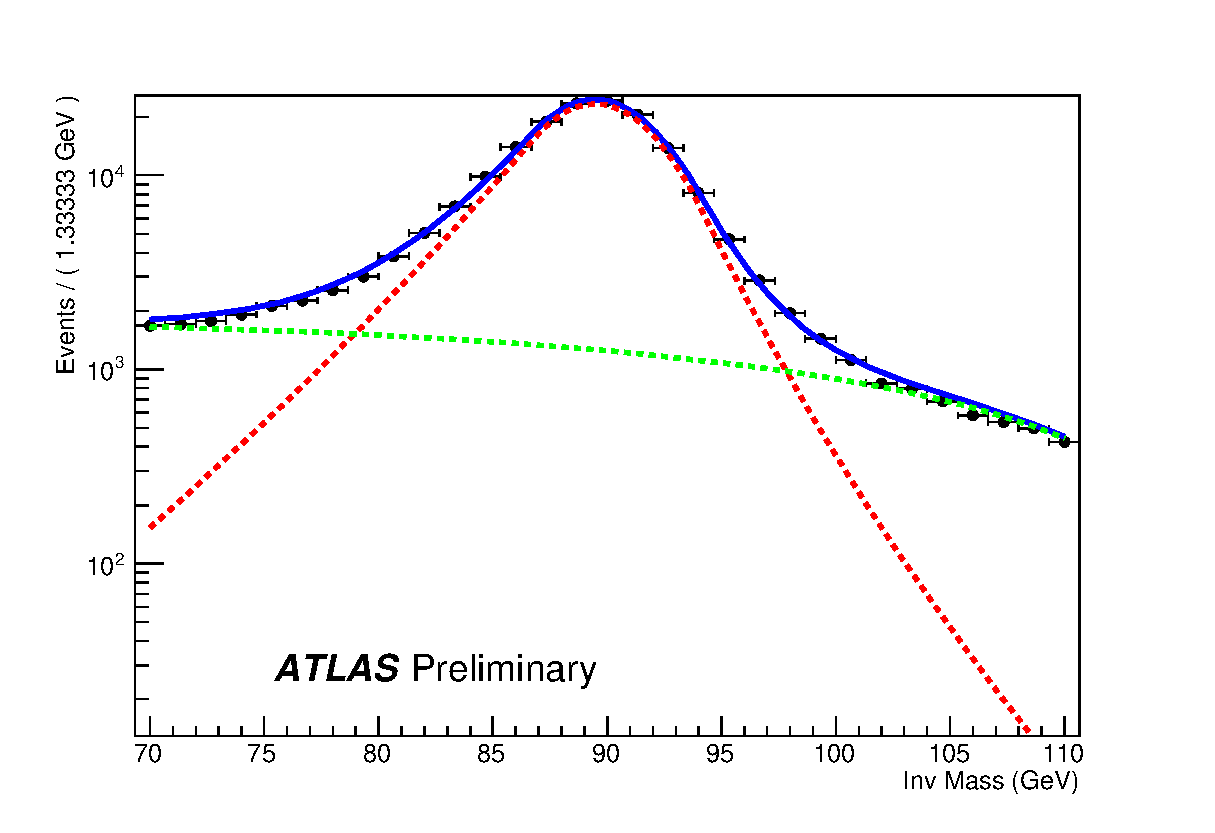
\includegraphics[scale=0.40]{d15_16_egam1_m_fit_h_m_eg_EE.eps}
	\end{subfigure}

	
	\caption{Fits de la masa invariante de los pares $ee$ (izquierda) y $e\gamma$ (derecha), reconstruídos en al región $EE$. La curva roja corresponde a la DSCB, la verde al polinomio de grado 2 y la azul a la combinación resultante de ambas.}
\label{fits_EE}
\end{figure}

